\documentclass[11pt,a4paper]{article}
\usepackage[margin=1in]{geometry}
\usepackage{setspace}
\usepackage{graphicx}
\usepackage{booktabs}
\usepackage{float}
\usepackage{hyperref}
\usepackage{enumitem}
\usepackage{xcolor}
\usepackage{fancyhdr}

\hypersetup{
  colorlinks=true,
  linkcolor=blue,
  urlcolor=blue,
  citecolor=blue
}

\pagestyle{fancy}
\fancyhf{}
\lhead{Retail Return Risk Modelling Report}
\rhead{Data Mining, Modelling and Analytics}
\cfoot{\thepage}

\setlength{\parskip}{0.5em}
\setlength{\parindent}{0pt}
\onehalfspacing

% ---------- Edit these metadata fields if needed ----------
\newcommand{\studentname}{Robert Tumushiime}
\newcommand{\accessno}{ACCESS-NO}
\newcommand{\programme}{MSc Data Science}
\newcommand{\courseyear}{Year 2, Semester 1}
\newcommand{\courseunit}{Data Mining, Modelling and Analytics}
\newcommand{\submissiondate}{19 March 2026}

% Application links
\newcommand{\streamliturl}{http://localhost:8502}
\newcommand{\apiurl}{http://127.0.0.1:8000}
\newcommand{\publicappurl}{http://localhost:8502}

\begin{document}

\begin{titlepage}
    \centering
    {\Large \textbf{Final Examination Report}}\\[1.2em]
    {\large \textbf{Retail Return Risk Prediction Using Structured Data and NLP}}\\[2em]

    \begin{tabular}{rl}
    \textbf{Student Name:} & \studentname \\
    \textbf{Access Number:} & \accessno \\
    \textbf{Programme:} & \programme \\
    \textbf{Course and Year:} & \courseyear \\
    \textbf{Course Unit:} & \courseunit \\
    \textbf{Submission Date:} & \submissiondate \\
    \end{tabular}

    \vfill

    \textbf{Submitted Requirements Included:}\\
    Notebook analysis, cleaned dataset, saved model artefact, predictions, NLP outputs,\\
    deployment scripts, and this final report with application link and user guidelines.

    \vfill
\end{titlepage}

\section{Executive Summary}
This project addresses a practical retail analytics problem: predicting whether a transaction line is likely to be returned or cancelled before dispatch. The solution combines structured transaction attributes (for example quantity, unit price, temporal fields, and country) with text mining over product descriptions. A complete pipeline was built covering data acquisition, cleaning, feature engineering, model comparison, threshold optimization, NLP analysis, and deployment design.

The final deployed inference stack uses a FastAPI backend and a Streamlit frontend. The selected production model is a HistGradientBoosting classifier saved in a joblib artefact together with an optimized decision threshold and feature metadata. Because the return class is highly imbalanced, model quality was evaluated with ROC-AUC and PR-AUC, with operational emphasis on return-class recall and F1 at the optimized threshold.

\section{Problem Definition and Business Objective}
Online retail operations frequently lose margin through returns, cancellations, reverse logistics, and handling costs. The analytical objective is to estimate return risk at transaction level using historical sales records and product-description text.

\textbf{Target variable:}
\begin{itemize}[leftmargin=1.5em]
    \item ReturnFlag = 1 if invoice number indicates cancellation (prefix C), else 0.
\end{itemize}

\textbf{Business objective:}
\begin{itemize}[leftmargin=1.5em]
    \item Predict risk before shipment.
    \item Support actions such as manual review, product-page refinement, and customer communication.
    \item Reduce cost of missed returns while preserving normal sales throughput.
\end{itemize}

\section{Dataset and Preparation}
The analysis used the UCI Online Retail dataset, containing over half a million transaction lines from an e-commerce business. The data contains both structured and unstructured signals:

\begin{itemize}[leftmargin=1.5em]
    \item Structured: Quantity, UnitPrice, InvoiceDate, CustomerID, Country, StockCode.
    \item Unstructured: Description text.
\end{itemize}

Cleaning and preparation followed an exam-ready reproducible process:
\begin{enumerate}[leftmargin=1.7em]
    \item Remove duplicates.
    \item Drop rows with missing critical fields.
    \item Standardize text fields and normalize descriptions.
    \item Remove invalid transaction values (UnitPrice \(\le 0\), Quantity \(= 0\)).
    \item Treat outliers through percentile clipping.
    \item Derive engineered features and save cleaned output as \texttt{Tumushiime.csv}.
\end{enumerate}

Figure~\ref{fig:eda} summarizes distributional characteristics and class imbalance in the cleaned dataset.

\begin{figure}[H]
    \centering
    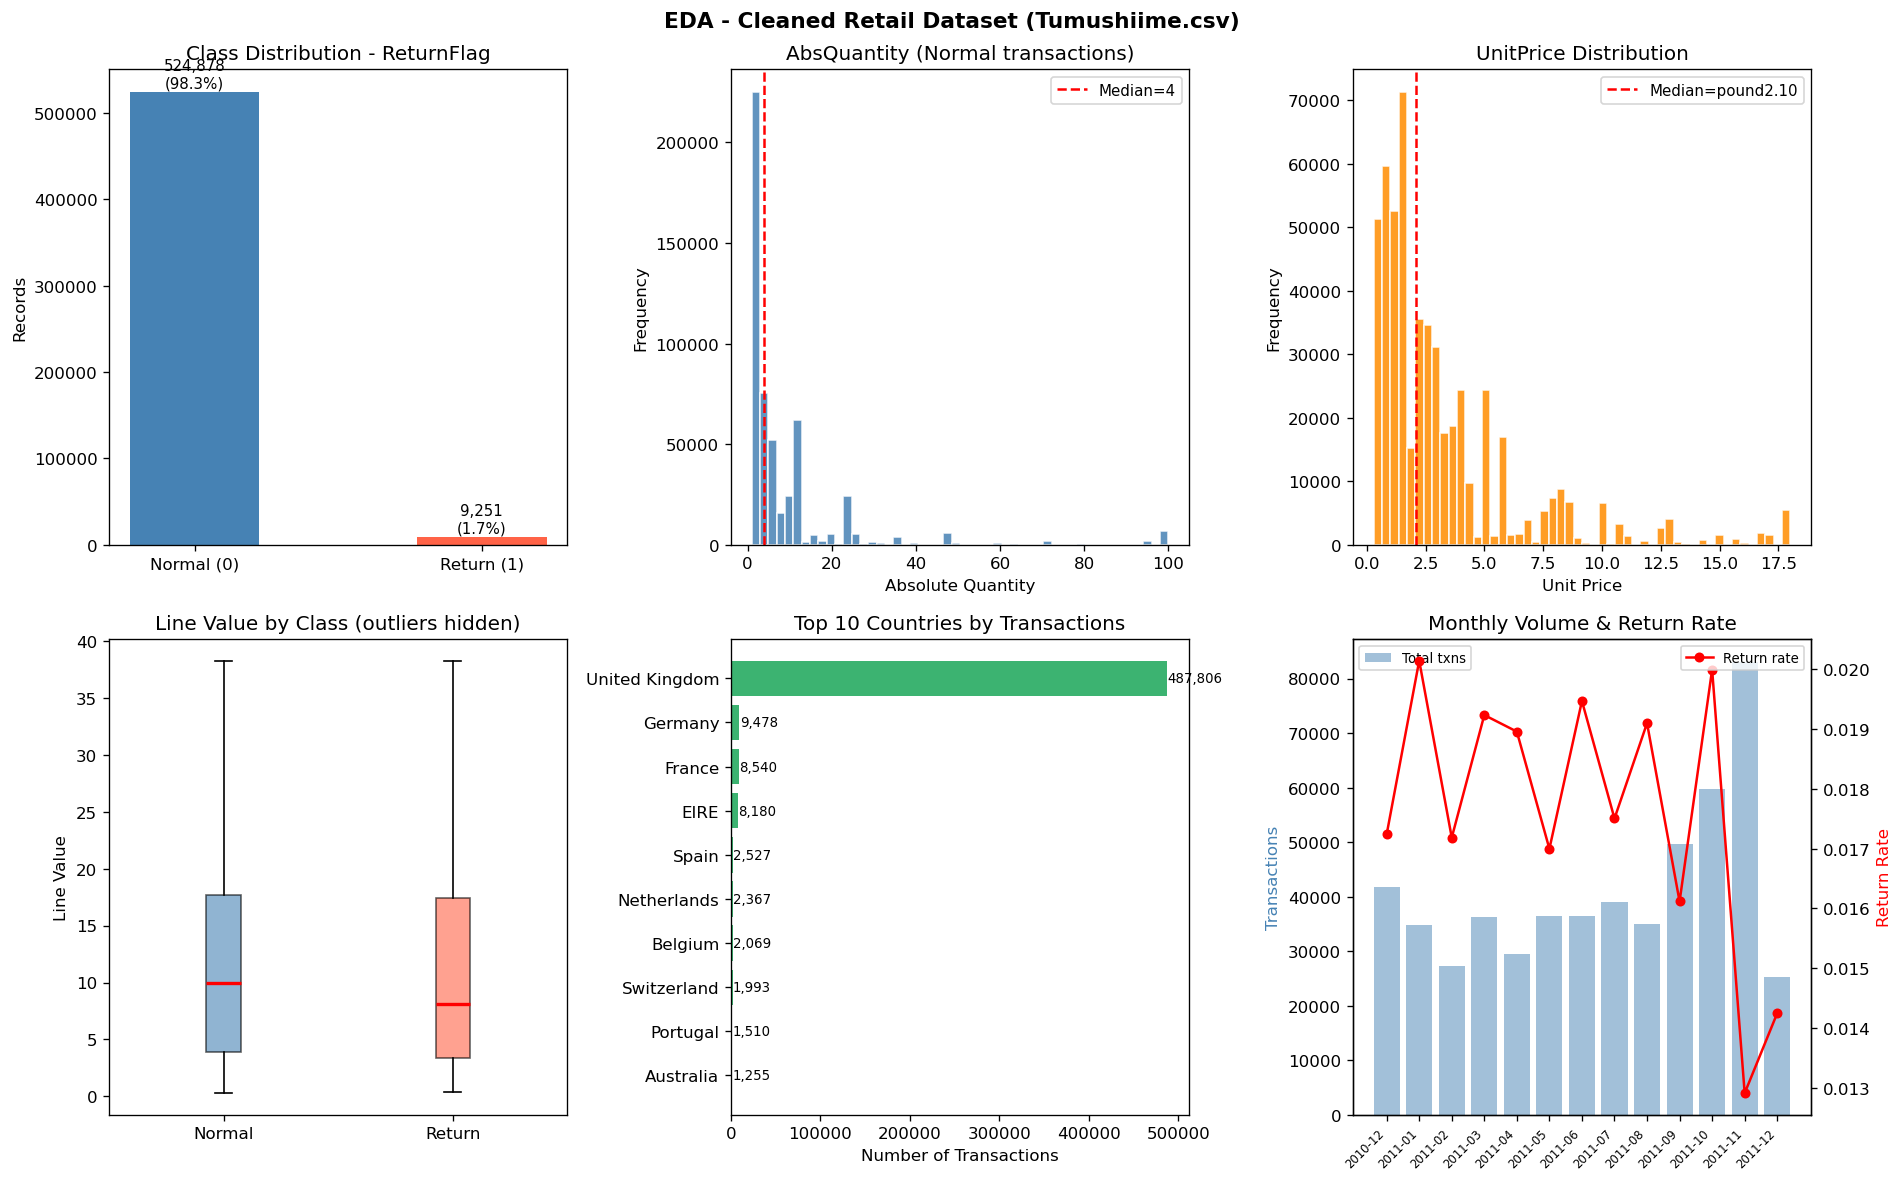
\includegraphics[width=0.98\textwidth]{Tumushiime_eda.png}
    \caption{EDA summary for cleaned retail dataset.}
    \label{fig:eda}
\end{figure}

\section{Feature Engineering and Modelling}
\subsection{Engineered Features}
The final model uses a combined feature space:
\begin{itemize}[leftmargin=1.5em]
    \item Numeric and categorical engineered features (9 fields):
    UnitPrice, AbsQuantity, LineValueAbs, InvoiceMonth, InvoiceWeekday, InvoiceHour, CustomerIDMissing, DescriptionLength, CountryEncoded.
    \item Text representation: TF-IDF with 200 features (unigrams and bigrams).
\end{itemize}

Random Forest importance analysis was used to validate useful predictors and explain feature contributions.

\begin{figure}[H]
    \centering
    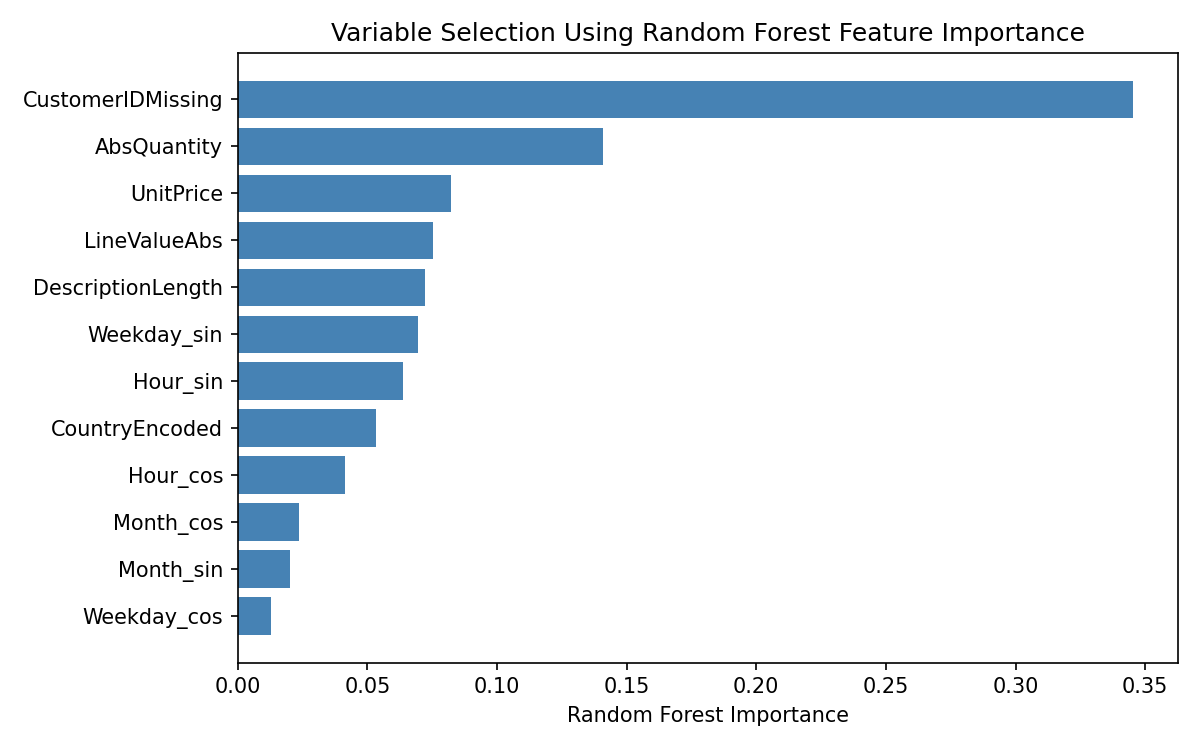
\includegraphics[width=0.82\textwidth]{Tumushiime_feature_importance.png}
    \caption{Numeric feature importance for variable selection and interpretation.}
    \label{fig:importance}
\end{figure}

\subsection{Model Comparison and Selection}
Three classifiers were trained and compared on a held-out test set:
\begin{itemize}[leftmargin=1.5em]
    \item Logistic Regression (baseline)
    \item Random Forest
    \item HistGradientBoosting (selected best model)
\end{itemize}

Since returns are rare, the primary evaluation metrics were ROC-AUC and PR-AUC. A probability threshold was tuned to improve return-class F1 for operational deployment.

\begin{table}[H]
\centering
\caption{Model comparison summary (actual notebook outputs).}
\begin{tabular}{lcccc}
\toprule
Model & ROC-AUC & PR-AUC & Return Recall & Return F1 \\
\midrule
Logistic Regression & 0.7445 & 0.0521 & 0.7135 & 0.0632 \\
Random Forest & 0.8371 & 0.1471 & 0.6822 & 0.1170 \\
HistGradientBoosting & 0.8594 & 0.2159 & 0.7459 & 0.1146 \\
\bottomrule
\end{tabular}
\end{table}

The selected production model is HistGradientBoosting because it achieved the best ROC-AUC and PR-AUC. The saved deployment threshold is 0.82499 from the model artefact.

\begin{figure}[H]
    \centering
    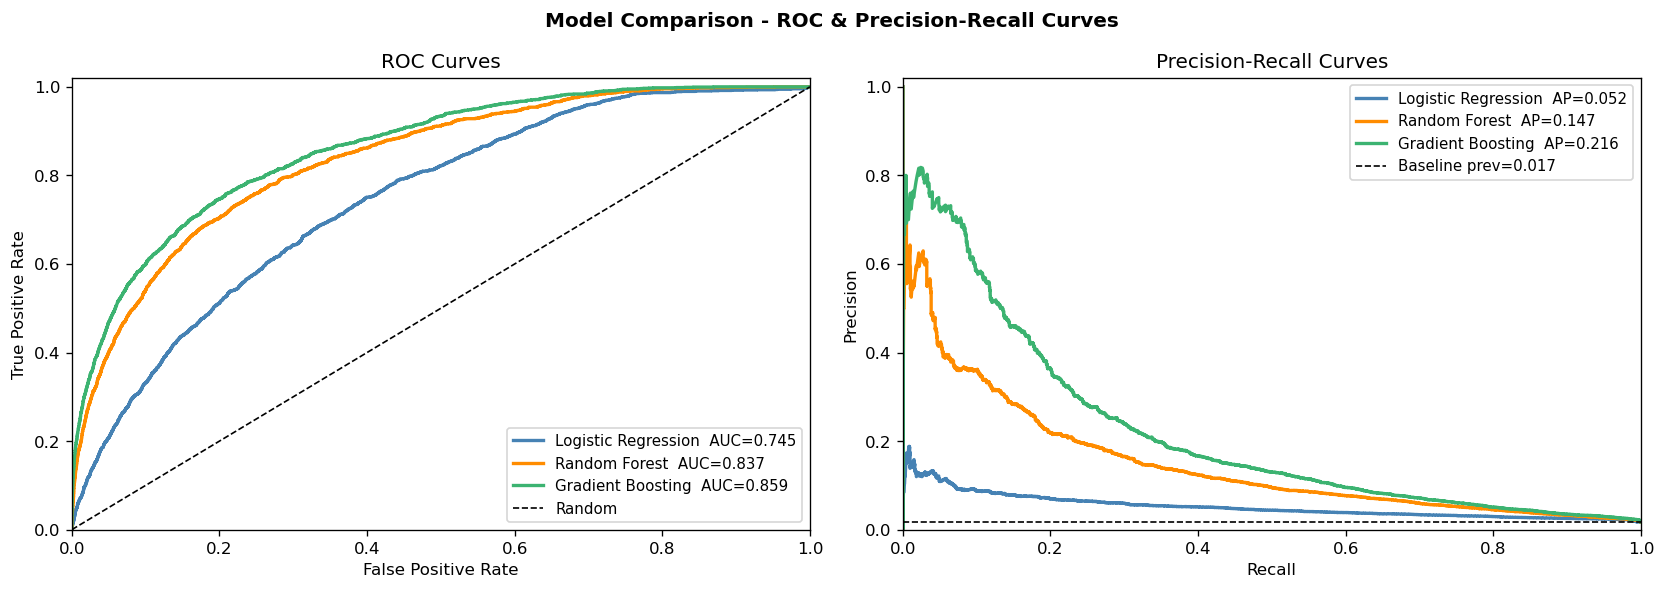
\includegraphics[width=0.95\textwidth]{Tumushiime_roc_pr_curves.png}
    \caption{ROC and Precision-Recall curves for model comparison.}
    \label{fig:curves}
\end{figure}

Final model artefact saved: \texttt{Tumushiime best model.joblib}.

\section{NLP Analysis and Insights}
To evaluate independent text signal, a text-only experiment was performed using product description text. The workflow used term frequency analysis, TF-IDF features, and Logistic Regression.

Key findings:
\begin{itemize}[leftmargin=1.5em]
    \item Product text provides meaningful predictive signal for return behavior.
    \item Administrative terms (for example manual, postage, adjustment-like language) are strongly associated with higher return risk contexts.
    \item Text-only modelling is useful but weaker than the fused structured + text model.
\end{itemize}

\begin{table}[H]
\centering
\caption{Text-only NLP model performance (actual notebook outputs).}
\begin{tabular}{lc}
\toprule
Metric & Value \\
\midrule
Accuracy & 0.3030 \\
Precision (Return) & 0.0194 \\
Recall (Return) & 0.7941 \\
F1 (Return) & 0.0380 \\
ROC-AUC & 0.6142 \\
PR-AUC & 0.0316 \\
\bottomrule
\end{tabular}
\end{table}

\begin{figure}[H]
    \centering
    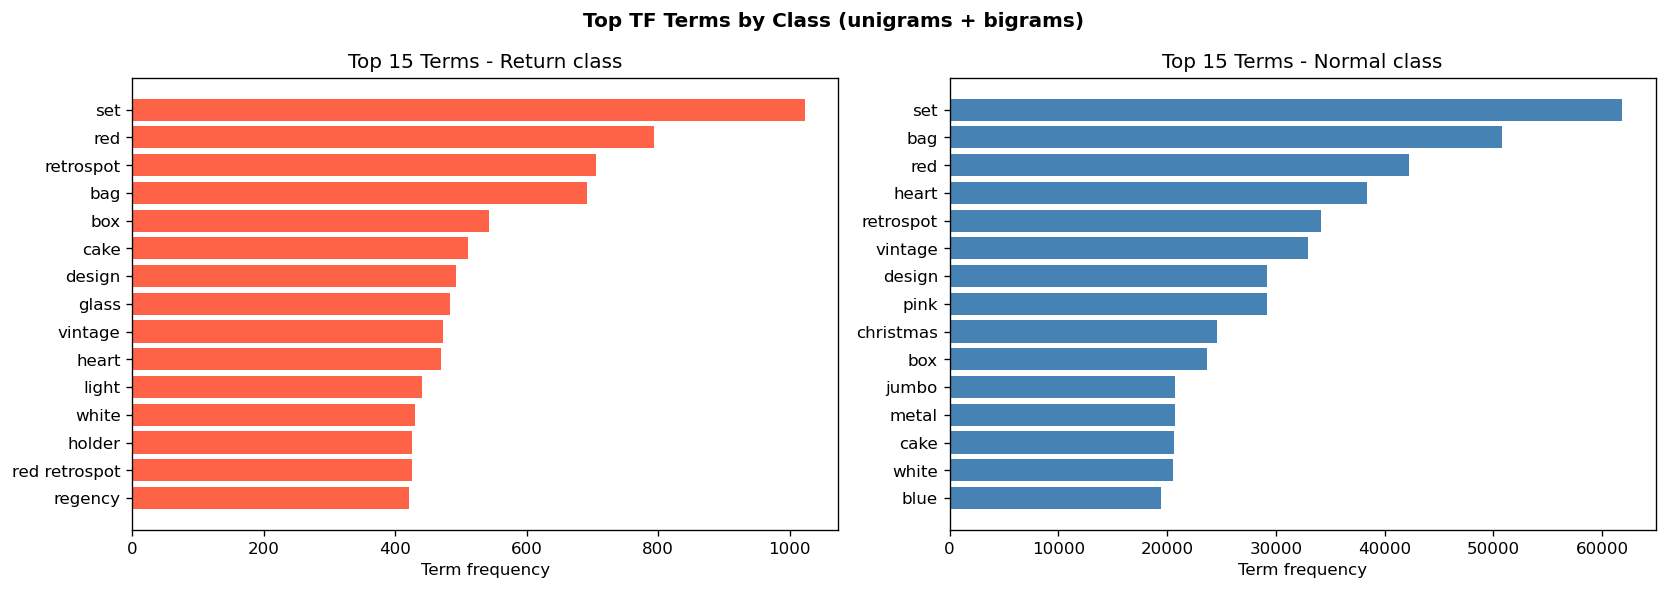
\includegraphics[width=0.95\textwidth]{Tumushiime_text_term_comparison.png}
    \caption{Top terms by return class versus normal class.}
    \label{fig:textterms}
\end{figure}

NLP output files include keyword coefficients and visualizations, such as \texttt{Tumushiime\_nlp\_keywords.csv}.

\section{Deployment Architecture and Application Link}
\subsection{Architecture}
The deployment design separates presentation and inference concerns:
\begin{itemize}[leftmargin=1.5em]
    \item \textbf{Frontend:} Streamlit app for single and batch predictions.
    \item \textbf{Backend:} FastAPI service with endpoints for health, model info, single predict, and batch predict.
    \item \textbf{Model artefact:} Joblib bundle containing model, threshold, and metadata.
\end{itemize}

\begin{figure}[H]
    \centering
    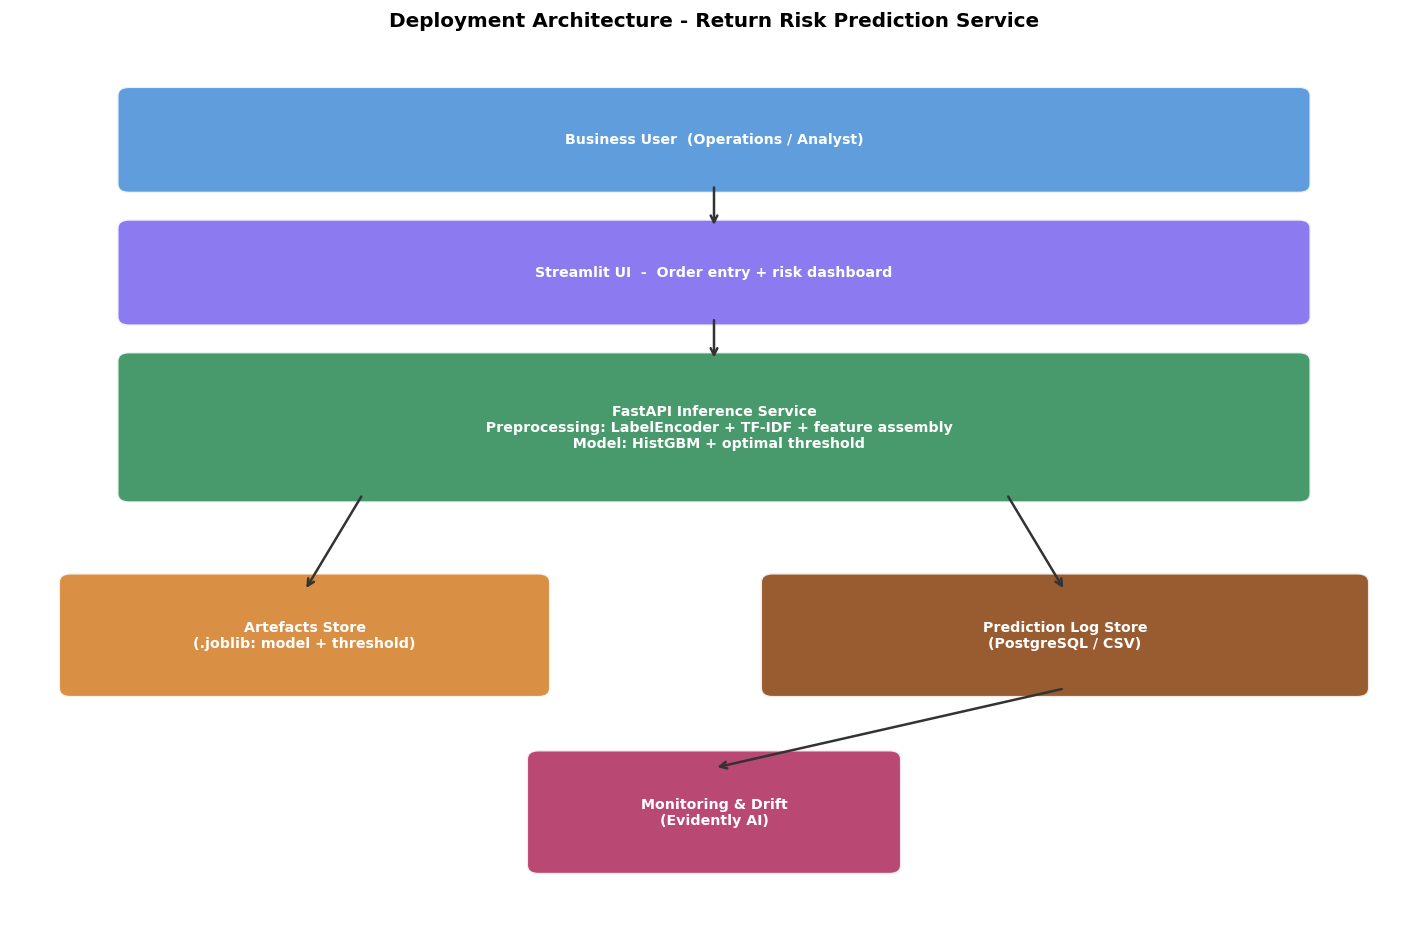
\includegraphics[width=0.95\textwidth]{Tumushiime_deployment_architecture.png}
    \caption{Deployment architecture for operational inference.}
    \label{fig:arch}
\end{figure}

\subsection{Running Application Link}
The application link included in this report is:
\begin{itemize}[leftmargin=1.5em]
    \item \textbf{Streamlit application link:} \url{\publicappurl}
    \item \textbf{Alternative local Streamlit URL:} \url{\streamliturl}
    \item \textbf{FastAPI base URL:} \url{\apiurl}
    \item \textbf{FastAPI interactive docs:} \url{\apiurl/docs}
\end{itemize}

\textit{Note: This Streamlit deployment is local to the running machine in the examination environment.}

\section{User Guidelines}
\subsection{How to use the web application}
\begin{enumerate}[leftmargin=1.7em]
    \item Open the Streamlit app URL: \url{\streamliturl}.
    \item Confirm the sidebar health check reports that API is running.
    \item Choose one workflow:
    \begin{itemize}[leftmargin=1.5em]
        \item \textbf{Single Prediction tab:} Enter product description and transaction details, then click Predict.
        \item \textbf{Batch Prediction tab:} Upload CSV and run batch scoring.
    \end{itemize}
    \item Read outputs:
    \begin{itemize}[leftmargin=1.5em]
        \item Return probability (continuous score)
        \item Predicted class label (RETURN or Normal Sale)
    \end{itemize}
\end{enumerate}

\subsection{Expected batch CSV columns}
For best compatibility, include at least:
\begin{itemize}[leftmargin=1.5em]
    \item Description
    \item UnitPrice
    \item Quantity
    \item Country
\end{itemize}
Optional fields accepted by defaults in UI/API:
\begin{itemize}[leftmargin=1.5em]
    \item InvoiceMonth, InvoiceWeekday, InvoiceHour, CustomerID
\end{itemize}

\subsection{API usage (optional for technical users)}
\begin{itemize}[leftmargin=1.5em]
    \item Single inference endpoint: \texttt{POST /predict}
    \item Batch inference endpoint: \texttt{POST /batch-predict}
    \item API docs and schema explorer: \url{\apiurl/docs}
\end{itemize}

\section{Ethical, Privacy, and Reliability Considerations}
Responsible operationalization requires safeguards in three areas:
\begin{itemize}[leftmargin=1.5em]
    \item \textbf{Ethics and fairness:} monitor subgroup error rates to reduce unjust impact.
    \item \textbf{Privacy and security:} apply data minimization, controlled access, and secure storage.
    \item \textbf{Reliability:} monitor drift and model quality over time, then retrain on schedule.
\end{itemize}

Predictions should support decisions, not replace policy and human oversight.

\section{Conclusion}
This project delivers a complete end-to-end retail return prediction solution: data preparation, feature engineering, model selection, NLP analysis, deployment scripts, and a working application interface. The final system is suitable for operational piloting and can be scaled with scheduled retraining, drift monitoring, and public hosting for wider access.

\vspace{1em}
\textbf{Submitted artefacts:}
\begin{itemize}[leftmargin=1.5em]
    \item Notebook: \texttt{Retail\_Final2.ipynb}
    \item Clean data: \texttt{Tumushiime.csv}
    \item Model: \texttt{Tumushiime best model.joblib}
    \item Predictions: \texttt{Tumushiime predictions.csv}
    \item NLP outputs: keyword CSV and comparison figures
    \item Deployment scripts: \texttt{ui\_streamlit.py}, \texttt{api\_service.py}
    \item Streamlit dependencies: \texttt{requirements.txt}
\end{itemize}

\end{document}
